\subsection{Organizing and planning (Roar)}

As a team, we have come to acknowledge the importance of organizing our workflow. At all meetings, a hearing is conducted involving a brief check-up of what was done last time, as well as what the next goals are. Once the goals are discussed and confirmed, the tasks are delegated. Depending on the tasks needed to be done, different approaches are used e.g. dividing up into subgroups or working as a whole. When implementing new features, it is more efficient to be divided up in smaller groups, to minimize code conflicts; while it is more efficient for everybody to work as a whole when larger design decisions are conducted. 

Often the working group (subgroup or whole) has a main programmer\footnote{This task often rotates, to keep one person from having full responsibility of coding.}, which implements the found solutions. The other member(s) confirm the solution and ensure that everything is covered.

To keep track of decisions, plans, schedules as well as assorted notes, we used a logbook. The logbook was kept in a shared text document. Here, we mostly wrote what we expected to work on at the start of the day as well as what we had finished by the end of the day, as conducted from the hearings. However, the logbook also contained possible features to implement, as well as several ideas on how to implement the different features. An excerpt from the logbook can be seen below.

\begin{figure}[H]
    \centering
    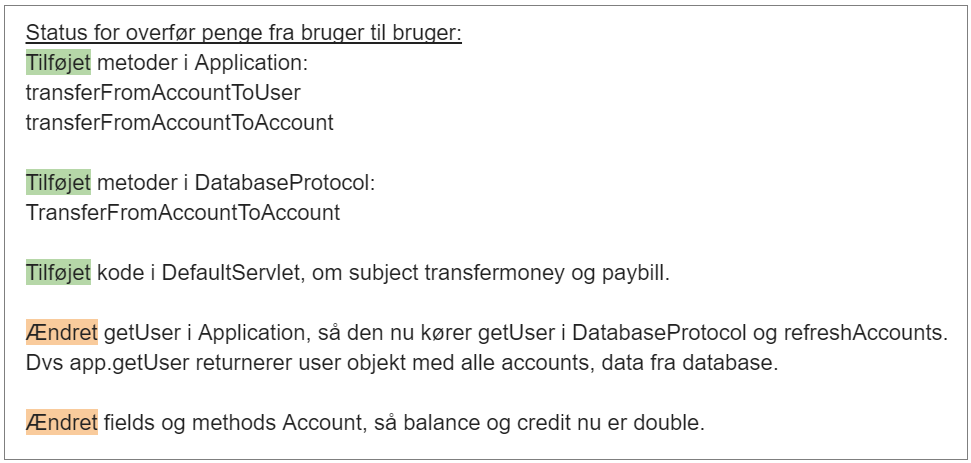
\includegraphics[width=0.7\textwidth]{figures/logbook2.PNG}
    \caption{An excerpt from the 30+ pages logbook. Application used: Google Docs.}
    \label{fig:logbook}
\end{figure}
